\documentclass{article}
\author{Jake Kolevas, Aidan Gresko}
\title{Main Simulator}
\date{\today}

\usepackage{times}
\usepackage{tcolorbox}
\usepackage{graphicx}
\usepackage{float}
\usepackage{amsmath}
\usepackage{siunitx}
\usepackage{tikz}
\usepackage{pgfplots}
\usepackage{float}
\pgfplotsset{compat=1.18}
\usetikzlibrary{shapes}

\begin{document}
	\maketitle
	
	\section{Overview}
	This project is to integrate a base power systems modeling package in Python, now with an added graphical user interface (GUI) for interactive simulation. The code establishes basic classes for power system components—buses, generators, conductors, geometries, and a top-level Circuit class to link them together. The Circuit class offers network building, equivalent distance calculation, and building of the network admittance matrix (Y-bus), which are crucial for load flow analysis.
	
	A primary new addition in this version is the MainWindow class, a PyQt6 graphical user interface (GUI) that allows users to define electrical circuits, execute powerflow simulations, and display results. The GUI has dynamic component addition (e.g., transformer, bus, loads), circuit configuration checking, and real-time feedback through text prints and matplotlib plots. It is combined with backend modules for circuit modeling, fault studies, and error handling, and the tool is more user-friendly for academic as well as real-world power system analysis.
	
	The modular architecture of the code allows for simultaneous development and future expansion, e.g., additional advanced modeling functionality and compatibility with other power system analysis software. The ultimate aim is to have a versatile, customized platform for debating power system concepts and elementary analysis, now with enhanced user interaction using the GUI.	
	
	\section{Class Diagram}
	
	\begin{figure}[H]
		\centering
		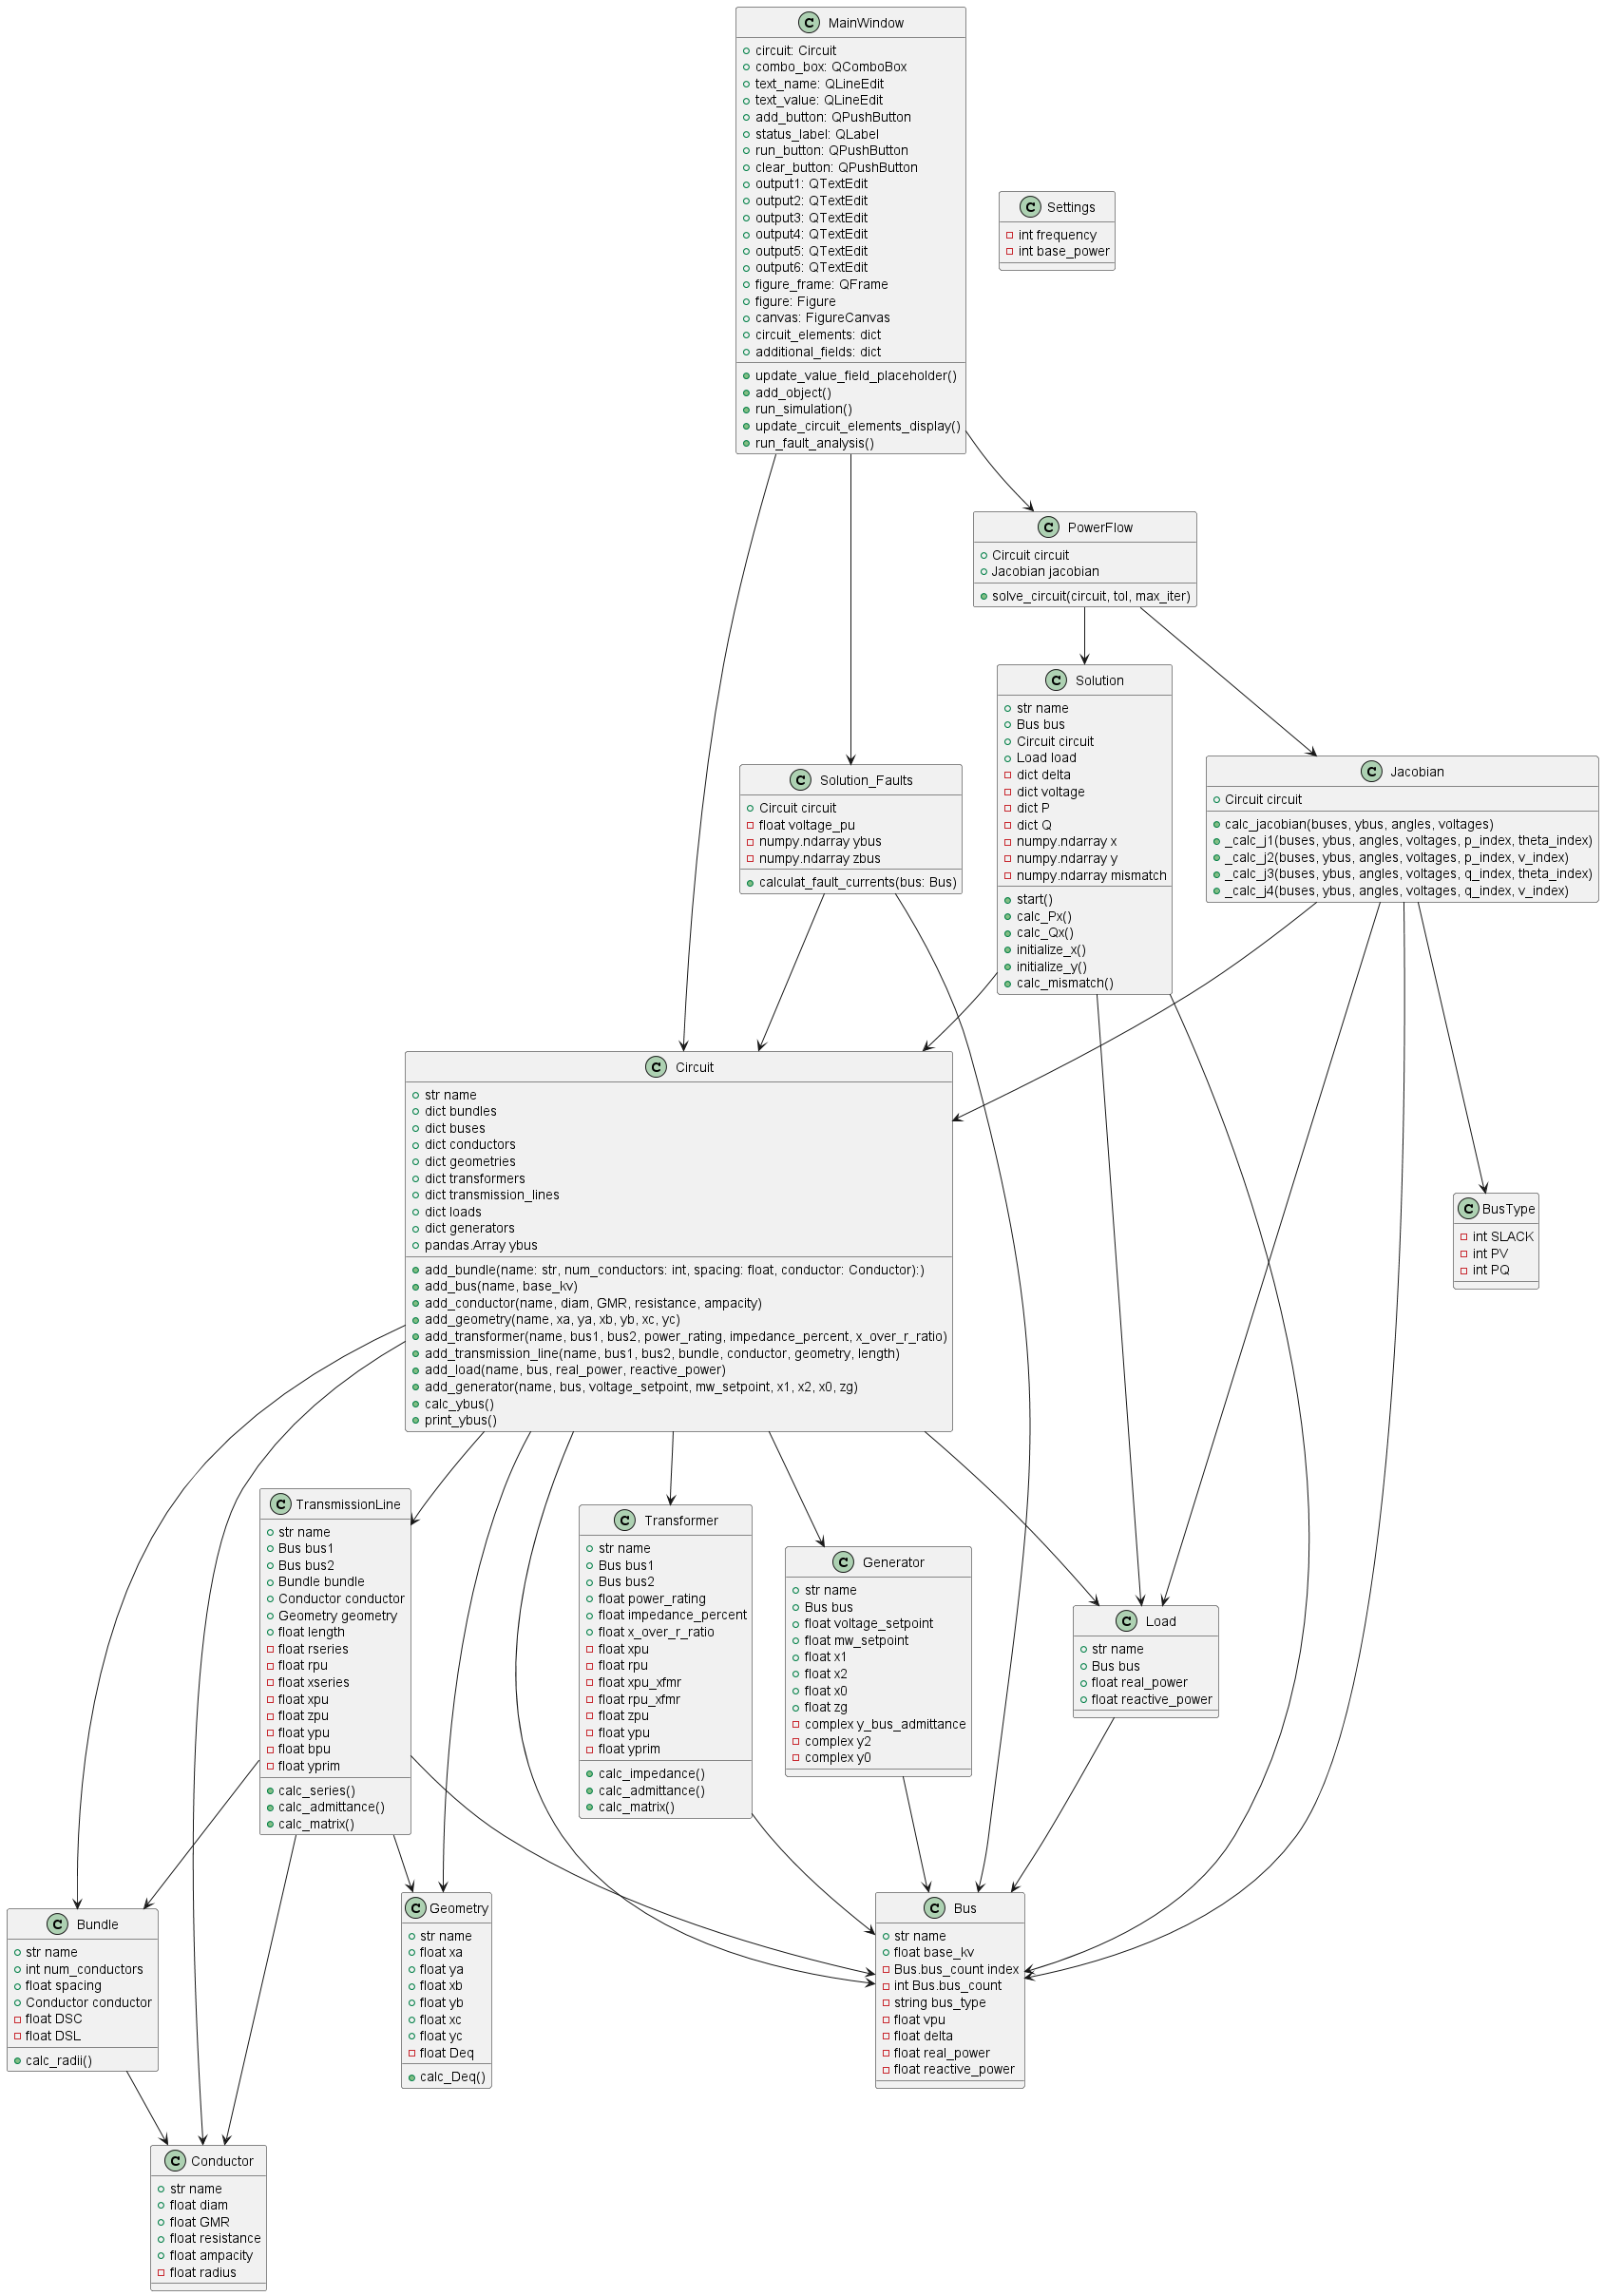
\includegraphics[scale=0.23]{../out/circuit/circuit.png}	
		\caption{Class Diagram for Project}
	\end{figure}
	
	\section{Classes}
	
	\subsection{Bundle}
	The Bundle class models a collection of conductors used in this simulation and calculates effective radii for resistance and inductance computations. This class is essential for modeling transmission lines, as it helps accurately compute effective radii for conductors arranged in bundles, affecting overall line behavior in analyses.
	
	\subsection{Bus}
	This Bus class is designed to model various types of buses within the power system, such as Slack, PV, and PQ buses. Each Bus instance is initialized with a name and base voltage (base\_kv). The class maintains a count of all Bus instances created using the class-level variable bus\_count. Key attributes include the bus type, voltage per unit (vpu), phase angle (delta), and power values (real\_power and reactive\_power). This class serves as a foundational component for simulating and analyzing power systems, enabling tracking of essential electrical characteristics for each bus.
	
	\subsection{Circuit}
	The Circuit class serves as a foundational component for modeling this power systems. It encapsulates the various elements that comprise a circuit—including buses, conductors, bundles, transformers, transmission lines, loads, and generators—providing a structured framework for representing and analyzing power flow. The class allows users to define and connect these components, storing their properties and relationships.  A key functionality is the calc\_ybus method, which computes the network admittance matrix (Y-bus) which is crucial for power system analysis. This class forms the basis for more complex power system studies, enabling simulations of load flow, fault analysis, and system stability.
	
	\subsection{Conductor}
	The Conductor class is designed to model electrical conductors by initializing them with key properties such as name, diameter (diam), geometric mean radius (GMR), resistance, and ampacity. Upon instantiation, these parameters are assigned to instance variables, and the radius is calculated by converting the diameter from a given unit to inches using a divisor of 24.
	
	\subsection{Generator}
	The Generator class models a generator component within this  power system. Each generator is initialized with a name for identification, an associated bus reference (Bus), a target voltage level (voltage\_setpoint), and a target power output in megawatts (mw\_setpoint).
	
	\subsection{Geometry}
	The Geometry class models a geometric figure defined by three points (A, B, and C) with their respective coordinates. Upon initialization, it calculates an attribute Deq, which is the average distance between each pair of these points. This is achieved using the distance formula to compute the lengths of sides AB, BC, and AC, then averaging them. The class is useful for scenarios requiring a measure of the average side length of a triangle formed by three points.
	
	\subsection{Jacobian}
	The Jacobian class performs the Jacobian matrix calculation for power flow analysis in power systems. It provides methods for calculating each of the four submatrices (J1, J2, J3, J4) that constitute the total Jacobian. These include the real power (P) and reactive power (Q) sensitivities due to variations in voltage angles ($\delta$) and voltage magnitudes (V). The class crosses the network buses, computing these sensitivities from the admittance matrix (Ybus) and voltage angle and magnitude current estimates. The calculated Jacobian is a critical input to iterative power flow solvers, including the Newton-Raphson solution, to determine power system operating conditions. The functions within this class calculate efficiently the partial derivatives utilized for power flow convergence.
	
	\subsection{Load}
	The Load class is an electrical load that is connected to some bus in the power system. Each load is described by a name, a pointer to the `Bus` that it is connected to, and its real\_power and reactive\_power demands (in Watts and VARs, respectively). This class simulates the action of power usage at a node in the network and is a key object to be utilized within power system simulation and analysis. It allows demand modeling of the electricity grid and must be done in order to conduct load flow, contingency, and other power calculations.
	
	\subsection{Powerflow}
	The PowerFlow class computes the voltage magnitudes and angles of every bus in a power system circuit through the Newton-Raphson power flow algorithm. It is initialized with a circuit object that defines the network topology and parameters, and the power flow solution is determined iteratively. The solve\_circuit method performs the primary power flow calculation with a tolerance (tol) and maximum iterations (max\_iter). It employs a Jacobian object to calculate the Jacobian matrix and then proceeds to use it to update bus voltage angles and magnitudes iteratively until a converged solution is reached. The function returns a dictionary containing the convergence status, number of iterations, final mismatch, calculated voltage magnitudes and angles, calculated real and reactive power injections, and a history of the mismatch values during the iteration process, providing a complete overview of the power flow solution.
	
	\subsection{Settings}
	The Settings class is a store of global parameters used throughout the power system analysis. It currently sets the system frequency (in Hertz) and base\_power (in MVA), base values used for per-unit calculation and conversion. This class provides simple modification and consistent application of these essential system parameters, with the benefit of code maintainability and the flexibility to represent different power system configurations. While presently constrained, it is designed to be extensible with more global settings as needed.
	
	\subsection{Seven Bus Power System}
	This Seven Bus Power System illustrates the development and solution of a power flow study on a typical electrical power system. It outlines the creation of a network model, including bus data, line data, and load data, in a Python setting. The code calculates the Jacobian matrix, a critical component of the power flow equations' solution, and utilizes a Newton-Raphson method to determine bus voltages and power injections. Additionally, the Seven Bus incorporates fault analysis capability, calculating fault currents and determining bus voltages under fault conditions. The code forms a foundation for power system behavior simulation, network stability verification, and contingency analysis, ultimately demonstrating an integrated approach to power system modeling and analysis.
	
	\subsection{Solution}
	This Solution class implements a Newton-Raphson power flow solver for power system network analysis. It solves bus voltages by iterative minimization of the mismatch between calculated and specified power injections, utilizing an external `circuit` object to define network data and topology. The solver accommodates various bus types (Slack, PV, PQ) and features base MVA scaling for normalized calculations. By converging to a solution, it provides valuable information on steady-state operation, including voltage profiles and power flows, and is therefore a key building block for power system analysis.
	
	\subsection{Solution Symmetric}
	\dots	
	
	\subsection{Transformer}
	The Transformer class models transformers in a power system, connecting two buses and calculating their electrical characteristics like impedance and admittance. It's essential for simulating power flow and analyzing the system's behavior in this simulation.
	
	\subsection{Transmission Line}
	The TransmissionLine class encapsulates the electrical characteristics of a power transmission line. It initializes with necessary components such as buses, conductors, bundles, geometry, and length. The class computes series impedance (rpu, xpu) and shunt admittance (bpu) using given formulas. These values are then used to construct an admittance matrix (yprim), essential for power flow analysis. This model allows detailed simulation of how electrical power is transmitted between two points in a power system.
	
	\subsection{MainWindow}
	The MainWindow class (PyQt6 UI Class) is the core GUI component of a powerflow simulation tool using PyQt6, where users can define electrical circuits, execute powerflow simulations, and visualize results. It features a dynamic user interface for adding components (e.g., buses, transformers, loads), circuit configuration checks, and simulation runs through Newton-Raphson algorithms. Outputs are bus voltages, power injections, convergence indicators, and fault analysis, displayed through text outputs and matplotlib plots. The course is coupled with backend modules for circuit modeling and fault studies with error handling and real-time feedback for user input.
	
	\section{Equations Used for Power Calculations}
	
	\subsection*{Bundle}
	1 conductor: \\
	\begin{align*}
		& DSC = r \\
		& DSL = GMR (\text{geometric mean radius})
	\end{align*}
	
	\noindent	
	2 conductors: \\
	\begin{align*}
		& DSC = \sqrt{r * s} \text{ -- r is radius and s is spacing} \\
		& DSL = \sqrt{GMR * s}
	\end{align*}
	
	\noindent	
	3 conductors: \\
	\begin{align*}
		& DSC = \sqrt[n]{r * s^2} \\
		& DSL = \sqrt[n]{GMR * s^2}
	\end{align*}
	
	\noindent
	4 conductors: \\
	\begin{align*}
		& DSC = 1.091 * (r * s^4)^{1/4} \\
		& DSL = 1.091 * (GMR * s^4)^{1/4}
	\end{align*}
	
	\noindent
	Where: \\
	- DSC is the equivalent diameter of a single circular conductor \\
	- DSL is the geometric mean radius of the bundle \\
	- r is the radius of individual conductors \\
	- s is the spacing between conductors 
	
	\subsection*{Circuit}
	
	\begin{align*}
		& \text{Y-Bus}[i,i] = \text{sum of all self-admittances at bus i} \\
		& \text{Y-Bus}[i,j] = \text{-sum of mutual admittances between buses i and j} \\
		& Z_{\text{transformer}} = \frac{\text{base\_voltage}^2}{\text{power\_rating}} * \frac{\text{impedance\_percent}}{100} \\
		& G_{\text{line}} = \text{conductance per unit length} * \text{length} \\
		& B_{\text{line}} = \text{susceptance per unit length} * \text{length} \\
		& Z_{\text{line}} = R + jX
	\end{align*}
	
	\subsection*{Generator}
	
	\begin{align*}
		& Y_1 = 1/jX_1 \\
		& Y_2 = 1/jX_2 \\
		& Y_0 = 1/(jX_0 + 3Zg)
	\end{align*}
	
	\noindent
	Where: \\
	- Y represents admittance (per unit or Siemens) \\
	- X represents reactance (per unit or Ohms) \\
	- Zg represents ground resistance (Ohms) \\
	- j is the imaginary unit $(\sqrt{-1})$ 
	
	\subsection*{Geometry}
	Euclidean Distance Formula: $d = \sqrt{(x_2 - x_1)^2 + (y_2 - y_1)^2}$ \\
	
	\subsection*{Jacobian}
	Active Power: 
	\[
	P_i = V_i \sum_{j=1}^{n} V_j[G_{ij} \cos(\delta_i - \delta_j) + B_{ij} \sin(\delta_i - \delta_j)]
	\]
	
	\noindent
	Reactive Power: 
	\[
	Q_i = V_i \sum_{j=1}^{n} V_j[G_{ij} \sin(\delta_i - \delta_j) - \cos(\delta_i - \delta_j)]
	\]
	
	\noindent
	Jacobian Sub-matrices: \\
	
	\noindent
	J1: 
	\[
	J1_{ij} = 
	\begin{cases}
		\hfill -V_i^2 \sum_{k \neq i} Y_{ik} \sin (\delta_i - \delta_k - \theta_{ik}) \text{ if } i = j  \\
		\hfill V_i V_j Y_i \sin(\delta_i - \delta_j - \theta_{ik}) \text{ if } i \neq j
	\end{cases}
	\]
	
	\noindent
	J2:
	\[
	J2_{ij} = 
	\begin{cases}
		\hfill V_i Y_{ii} \cos(\delta_i - \delta_i - \theta_{ii}) + V_i \sum_{k \neq i} Y_{ik} \cos(\delta_i - \delta_k - \theta_{ik}) \text{ if } i = j \\
		\hfill V_i Y_{ij} \cos(\delta_i - \delta_j - \theta_{ij}) \text{ if } i \neq j
	\end{cases}
	\]
	
	\noindent
	J3: 
	\[
	J3_{ij} = 
	\begin{cases}
		\hfill V_i^2 \sum_{k \neq i} Y_{ik} \cos(\delta_i - \delta_k - \theta_{ik}) \text{ if } i = j \\
		\hfill -V_i V_j Y_{ij} \cos(\delta_i - \delta_j - \theta_{ij}) \text{ if } i \neq j
	\end{cases}
	\]
	
	\noindent
	J4: 
	\[
	J4_{ij} = 
	\begin{cases}
		\hfill -V_i Y_{ii} \sin(\delta_i - \delta_i - \theta_{ii}) + V_i \sum_{k \neq i} Y_{ik} \sin(\delta_i - \delta_k - \theta_{ik}) \text{ if } i = j \\
		\hfill V_i Y_{ij} \sin(\delta_i - \delta_j - \theta_{ij}) \text{ if } i \neq j
	\end{cases}
	\]
	
	\noindent
	Where: \\
	- $V_i$ and $V_j$: Voltage magnitudes at buses i and j \\
	- $G_{ij}$ and $B_{ij}$: Real and imaginary parts of the admittance between buses i and j \\
	- $Y_{ii}$: Admittance between buses i and j, where $Y_{ij} = G_{ij} + j B_{ij}$ \\
	- $\delta_i$ and $\delta_j$: Phase angles at buses i and j \\
	- $\theta_{ij}$: Phase angle of the admittance $Y_{ij}$
	
	\subsection*{PowerFlow}
	Newton-Raphson Method: 
	\[
	J \cdot dx = -\text{mismatch}
	\]
	
	\noindent
	Angle and Voltage Corrections: 
	\[
	\Delta \theta_{i}^{k+1} = \Delta \theta_i^k + dx_i
	\]
	
	\subsection*{Solution}
	Active Power Mismatch: 
	\[
	\Delta P_i = P_{spec,i} - P_i
	\]
	
	\noindent	
	Reactive Power Mistmatch: 
	\[
	\Delta Q_i = Q_{spec,i} - Q_i
	\]
	
	\subsection*{Solution Faults}
	Inverse Matrix: 
	\[
	Z_{bus} = (Y_{bus})^{-1}
	\]
	
	\noindent
	Fault Current at Bus: 
	\[
	I_f(n) = \frac{V_{pu}}{Z_{nn}}
	\]
	
	\noindent
	Bus Voltage Post-Fault: 
	\[
	V_k = (1 - \frac{ Z_{kn} }{ Z_{nn} }) \times V_{pu}
	\]
	
	\subsection*{Transformer}
	\noindent
	Transformer Impedance:
	\[ Z_{pu} = \frac{Z_\%}{100} \cdot \frac{S_{\text{base}}}{S_{\text{transformer}}} \angle{\theta} \]
	where \( \theta = \tan^{-1}(X/R) \). \\
	
	\noindent
	Transformer Admittance:
	\[ Y_{pu} = \frac{1}{Z_{pu}} \]
	
	\noindent
	Transformer Y-Bus Matrix:
	\[ [Y_{\text{Bus}}] = 
	\begin{bmatrix}
		Y_{11} & -Y_{12} \\
		-Y_{21} & Y_{22}
	\end{bmatrix} \]
	where \( -Y_{12} = -Y_{21} \).
	
	\subsection*{Transmission Line}
	Series Resistance Calculation: 
	\[
	R_{series} = (\frac{p}{n}) \times L
	\]
	
	\noindent	
	Series Reactance Calculation: 
	\[
	X_{series} = 2 \pi f \times \mu_0 \times \log(\frac{D_{eq}}{D_{SL}}) \times L
	\]
	
	\noindent
	Per Unit Impedance: 
	\[
	Z_{pu} = R_{pu} + j X_{pu}
	\]
	
	\noindent
	Shunt Admittance Calculation: 
	\[
	B_{shunt} = 2 \pi f \times \frac{\epsilon_0}{\log(\frac{D_{eq}}{D_{SC}})} \times L
	\]
	
	\noindent
	Per Unit Shunt Admittance Calculation: 
	\[
	B_{pu} = \frac{B_{shunt}}{Y_{base}}
	\]
	
	\noindent	
	Prim Matrix Calculation:
	\[
	Y' = \begin{bmatrix}
		Y_p + B/2 & -Y_p \\
		-Y_p & Y_p + B/2
	\end{bmatrix}
	\]
	
	\noindent
	Where: \\
	- \(Y_p\) is the per unit admittance due to series resistance and reactance. \\
	- \(B\) is the shunt conductance (real part of admittance).
	
	\section{Example Problem with Solution}
	
	This section presents a practical example of power flow analysis using the developed graphical user interface. We will analyze a 7-bus power system, calculate power flows, and interpret the results.
	
	\subsection{Problem Statement}
	
	Consider the 7-bus power system shown in Figure \ref{fig:seven_bus_system} with the following parameters:
	
	\begin{figure}[H]
		\centering
		% Required packages in preamble: 
		% \usepackage{tikz}
		% \usepackage{pgfplots}
		% \pgfplotsset{compat=1.18}
		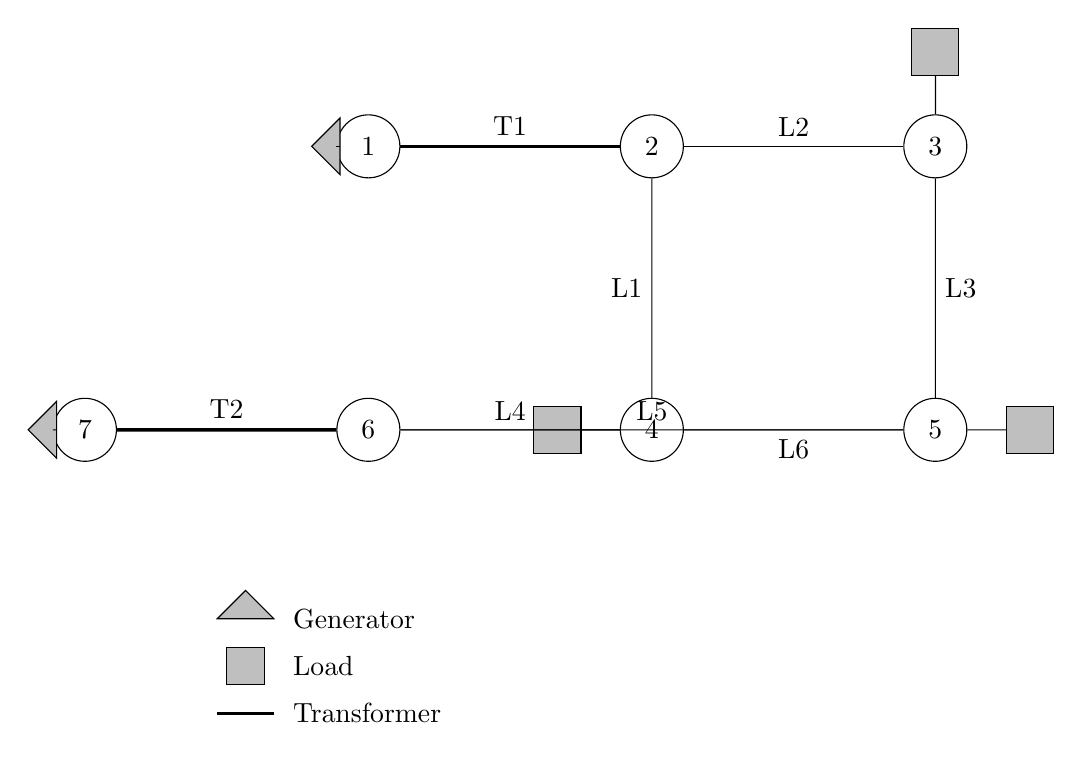
\begin{tikzpicture}[
			bus/.style={circle, draw, minimum size=0.8cm, inner sep=0pt},
			load/.style={rectangle, draw, minimum width=0.6cm, minimum height=0.6cm},
			scale=1.2
			]
			
			% Buses
			\node[bus] (bus1) at (0,0) {1};
			\node[bus] (bus2) at (3,0) {2};
			\node[bus] (bus3) at (6,0) {3};
			\node[bus] (bus4) at (3,-3) {4};
			\node[bus] (bus5) at (6,-3) {5};
			\node[bus] (bus6) at (0,-3) {6};
			\node[bus] (bus7) at (-3,-3) {7};
			
			% Generator symbols - using direct drawing to avoid TikZ library requirements
			\draw[fill=lightgray] (-0.3,0.3) -- (-0.3,-0.3) -- (-0.6,0) -- cycle;
			\draw (-0.3,0) -- (bus1);
			
			% Generator at Bus 7
			\draw[fill=lightgray] (-3.3,-2.7) -- (-3.3,-3.3) -- (-3.6,-3) -- cycle;
			\draw (-3.3,-3) -- (bus7);
			
			% Transformers
			\draw[very thick] (bus1) -- node[above, sloped] {T1} (bus2);
			\draw[very thick] (bus6) -- node[above, sloped] {T2} (bus7);
			
			% Loads at Bus 3
			\node[load, fill=lightgray] (load3) at (6,1) {};
			\draw (load3) -- (bus3);
			
			% Load at Bus 4
			\node[load, fill=lightgray] (load4) at (2,-3) {};
			\draw (load4) -- (bus4);
			
			% Load at Bus 5
			\node[load, fill=lightgray] (load5) at (7,-3) {};
			\draw (load5) -- (bus5);
			
			% Transmission Lines
			\draw (bus2) -- node[above] {L2} (bus3);
			\draw (bus2) -- node[left] {L1} (bus4);
			\draw (bus3) -- node[right] {L3} (bus5);
			\draw (bus4) -- node[below] {L6} (bus5);
			\draw (bus4) -- node[above] {L4} (bus6);
			\draw (bus5) -- node[above, sloped] {L5} (bus6);
			
			% Legend
			\draw[fill=lightgray] (-1,-5) -- (-1.6,-5) -- (-1.3,-4.7) -- cycle;
			\node[right] at (-0.9,-5) {Generator};
			\node[load, fill=lightgray, scale=0.8] at (-1.3,-5.5) {};
			\node[right] at (-0.9,-5.5) {Load};
			\draw[very thick, -] (-1.6,-6) -- (-1,-6);
			\node[right] at (-0.9,-6) {Transformer};
			
		\end{tikzpicture}
		\caption{7-Bus Power System}
		\label{fig:seven_bus_system}
	\end{figure}
	
	\noindent \textbf{Bus Data:}
	\begin{itemize}
		\item Bus 1: Slack bus, voltage $V_1 = 1.0 \angle 0^\circ$ pu, base voltage 20 kV
		\item Bus 2: Load bus (PQ), base voltage 230 kV
		\item Bus 3: Load bus (PQ), base voltage 230 kV
		\item Bus 4: Load bus (PQ), base voltage 230 kV
		\item Bus 5: Load bus (PQ), base voltage 230 kV
		\item Bus 6: Load bus (PQ), base voltage 230 kV
		\item Bus 7: Generator bus (PV), voltage magnitude $V_7 = 1.0$ pu, $P_{G7} = 200$ MW, base voltage 18 kV
	\end{itemize}
	
	\noindent \textbf{Load Data:}
	\begin{itemize}
		\item Bus 3: $P_{L3} = 110$ MW, $Q_{L3} = 50$ MVAR
		\item Bus 4: $P_{L4} = 100$ MW, $Q_{L4} = 70$ MVAR
		\item Bus 5: $P_{L5} = 100$ MW, $Q_{L5} = 65$ MVAR
	\end{itemize}
	
	\noindent \textbf{Transformer Data:}
	\begin{table}[H]
		\centering
		\begin{tabular}{ccccc}
			\hline
			\textbf{Name} & \textbf{From Bus} & \textbf{To Bus} & \textbf{MVA Rating} & \textbf{Impedance (\%)} \\
			\hline
			T1 & 1 & 2 & 125 & 8.5 \\
			T2 & 6 & 7 & 200 & 10.5 \\
			\hline
		\end{tabular}
		\caption{Transformer Parameters}
		\label{tab:transformer_data}
	\end{table}
	
	\noindent \textbf{Transmission Line Data:}
	\begin{table}[H]
		\centering
		\begin{tabular}{ccccc}
			\hline
			\textbf{Line} & \textbf{From Bus} & \textbf{To Bus} & \textbf{Conductor} & \textbf{Length (mi)} \\
			\hline
			L1 & 2 & 4 & C1 & 10 \\
			L2 & 2 & 3 & C1 & 25 \\
			L3 & 3 & 5 & C1 & 20 \\
			L4 & 4 & 6 & C1 & 20 \\
			L5 & 5 & 6 & C1 & 10 \\
			L6 & 4 & 5 & C1 & 35 \\
			\hline
		\end{tabular}
		\caption{Transmission Line Parameters}
		\label{tab:line_data}
	\end{table}
	
	\noindent \textbf{Conductor Data:}
	\begin{itemize}
		\item Type: C1
		\item Resistance: 0.642 $\Omega$/mile
		\item Reactance: 0.0217 $\Omega$/mile
		\item Diameter: 0.385 inches
		\item Ampacity: 460 A
	\end{itemize}
	
	\noindent \textbf{Bundle Configuration:}
	\begin{itemize}
		\item Bundle B1: 2 conductors of type C1 with 1.5 ft spacing
	\end{itemize}
	
	\noindent \textbf{Geometry Configuration:}
	\begin{itemize}
		\item Geometry G1: Horizontal configuration with phase positions at (0,0), (18.5,0), and (37,0) ft
	\end{itemize}
	
	The objective is to determine:
	\begin{enumerate}
		\item The voltage magnitude and angle at each bus
		\item Power flow in all transmission lines and transformers
		\item Generator power output at the slack bus
		\item System losses
	\end{enumerate}
	
	\subsection{Solution Approach}
	
	To solve this power flow problem using our GUI application, we follow these steps:
	
	\begin{enumerate}
		\item Input all bus data, including voltage levels and bus types
		\item Add conductor data and bundle configurations
		\item Add geometry configurations for transmission lines
		\item Input transformer parameters
		\item Add transmission lines with proper connections
		\item Specify the load values
		\item Configure the generators
		\item Run the Newton-Raphson power flow algorithm
		\item Analyze the results
	\end{enumerate}
	
	The following sections detail this process and show the resulting outputs.
	
	\subsection{Implementation in the GUI}
	
	Using the GUI application, we enter the components as shown in the sequence below:
	
	\begin{table}[H]
		\centering
		\begin{tabular}{ccl}
			\hline
			\textbf{Component Type} & \textbf{Name} & \textbf{Value} \\
			\hline
			Bus & Bus1 & 20,Slack Bus \\
			Bus & Bus2 & 230,PQ Bus \\
			Bus & Bus3 & 230,PQ Bus \\
			Bus & Bus4 & 230,PQ Bus \\
			Bus & Bus5 & 230,PQ Bus \\
			Bus & Bus6 & 230,PQ Bus \\
			Bus & Bus7 & 18,PV Bus \\
			Transformer & T1 & Bus1,Bus2,125,8.5 \\
			Transformer & T2 & Bus6,Bus7,200,10.5 \\
			Conductor & C1 & 0.642,0.0217,0.385,460 \\
			Bundle & B1 & 2,1.5,C1 \\
			Geometry & G1 & 0,0,18.5,0,37,0 \\
			Transmission Line & L1 & Bus2,Bus4,B1,C1,G1,10 \\
			Transmission Line & L2 & Bus2,Bus3,B1,C1,G1,25 \\
			Transmission Line & L3 & Bus3,Bus5,B1,C1,G1,20 \\
			Transmission Line & L4 & Bus4,Bus6,B1,C1,G1,20 \\
			Transmission Line & L5 & Bus5,Bus6,B1,C1,G1,10 \\
			Transmission Line & L6 & Bus4,Bus5,B1,C1,G1,35 \\
			Load & Load3 & Bus3,110,50 \\
			Load & Load4 & Bus4,100,70 \\
			Load & Load5 & Bus5,100,65 \\
			Generator & G1 & Bus1,1.0,0.0,0.12,0.14,0.05,0 \\
			Generator & G7 & Bus7,1.0,200,0.12,0.14,0.05,0 \\
			\hline
		\end{tabular}
		\caption{Component Input Sequence for GUI}
		\label{tab:gui_inputs}
	\end{table}
	
	\subsection{Power Flow Results}
	
	After running the simulation, the GUI generates the following results:
	
	\subsubsection{Bus Voltages}
	
	\begin{table}[H]
		\centering
		\begin{tabular}{cccc}
			\hline
			\textbf{Bus} & \textbf{Voltage Magnitude (pu)} & \textbf{Voltage Angle (degrees)} & \textbf{Type} \\
			\hline
			Bus1 & 1.0000 & 0.00 & Slack \\
			Bus2 & 0.9360 & -4.46 & PQ \\
			Bus3 & 0.9194 & -5.49 & PQ \\
			Bus4 & 0.9288 & -4.72 & PQ \\
			Bus5 & 0.9256 & -4.86 & PQ \\
			Bus6 & 0.9385 & -3.97 & PQ \\
			Bus7 & 1.0000 & 2.08 & PV \\
			\hline
		\end{tabular}
		\caption{Bus Voltage Results}
		\label{tab:voltage_results}
	\end{table}
	
	\subsubsection{Power Flow in Lines and Transformers}
	
	\begin{table}[H]
		\centering
		\begin{tabular}{ccc}
			\hline
			\textbf{Bus} & \textbf{Active Power (MW)} & \textbf{Reactive Power (MVAR)} \\
			\hline
			Bus1 & 116.36 & 87.13 \\
			Bus2 & 0.00 & 0.00 \\
			Bus3 & -110.00 & -50.00 \\
			Bus4 & -100.00 & -70.00 \\
			Bus5 & -100.00 & -65.00 \\
			Bus6 & 0.00 & 0.01 \\
			Bus7 & 200.00 & 107.66 \\
			\hline
		\end{tabular}
		\caption{Bus Power Injections}
		\label{tab:power_injections}
	\end{table}
	
	\subsubsection{Generator Outputs}
	
	\begin{table}[H]
		\centering
		\begin{tabular}{cccc}
			\hline
			\textbf{Bus} & \textbf{Generator} & \textbf{Active Power (MW)} & \textbf{Reactive Power (MVAR)} \\
			\hline
			Bus1 & G1 & 116.36 & 87.13 \\
			Bus7 & G7 & 200.00 & 107.66 \\
			\hline
		\end{tabular}
		\caption{Generator Power Outputs}
		\label{tab:generator_results}
	\end{table}
	
	\subsubsection{System Losses}
	
	\begin{table}[H]
		\centering
		\begin{tabular}{cc}
			\hline
			\textbf{Type} & \textbf{Value} \\
			\hline
			Active Power Losses & 6.36 MW \\
			Reactive Power Losses & 9.80 MVAR \\
			\hline
		\end{tabular}
		\caption{System Losses}
		\label{tab:losses}
	\end{table}
	
	\subsubsection{Convergence}
	
	The power flow solution converged in 2 iterations with a maximum power mismatch of $5.3 \times 10^{-5}$ pu.
	
	\subsection{Analysis of Results}
	
	\begin{enumerate}
		\item \textbf{Voltage Profile}: All bus voltages are within acceptable limits (0.92-1.05 pu), with the lowest voltage at Bus 3 (0.9194 pu).
		
		\item \textbf{Power Flow Distribution}: The power flows from the two generators (at Bus 1 and Bus 7) to the three load centers (at Bus 3, Bus 4, and Bus 5). The generators at Bus 1 and Bus 7 supply 116.36 MW and 200 MW respectively.
		
		\item \textbf{Generator Outputs}: The slack bus (Bus 1) generates 116.36 MW and 87.13 MVAR to balance the system, while the PV bus (Bus 7) maintains its scheduled 200 MW output with 107.66 MVAR reactive power support.
		
		\item \textbf{System Losses}: The total system losses are 6.36 MW (2.0% of total generation) and 9.80 MVAR, which is reasonable for this transmission system.
		
		\item \textbf{Load Balance}: Total generation (316.36 MW) equals the sum of total load (310 MW) and system losses (6.36 MW), confirming power balance.
		
		\item \textbf{Fast Convergence}: The solution converged in only 2 iterations, indicating good numerical stability of the model.
	\end{enumerate}
	
	\subsection{Visualization}
	
	Figure \ref{fig:voltage_profile} shows the voltage profile across the system, providing a visual representation of the voltage variations.
	
	\begin{figure}[H]
		\centering
		% Required packages in preamble: 
		% \usepackage{tikz}
		% \usepackage{pgfplots}
		% \pgfplotsset{compat=1.18}
		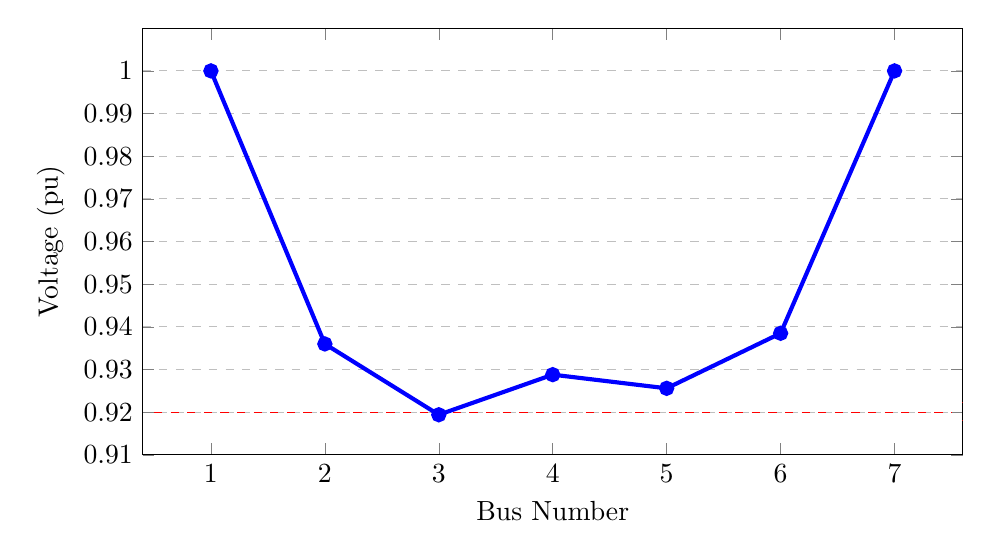
\begin{tikzpicture}
			\begin{axis}[
				xlabel={Bus Number},
				ylabel={Voltage (pu)},
				xtick={1,2,3,4,5,6,7},
				ytick={0.91,0.92,0.93,0.94,0.95,0.96,0.97,0.98,0.99,1.00},
				ymin=0.91, ymax=1.01,
				ymajorgrids=true,
				grid style=dashed,
				width=12cm,
				height=7cm
				]
				
				\addplot[
				color=blue,
				mark=*,
				line width=1.5pt
				]
				coordinates {
					(1,1.0000)
					(2,0.9360)
					(3,0.9194)
					(4,0.9288)
					(5,0.9256)
					(6,0.9385)
					(7,1.0000)
				};
				
				\draw[dashed, red] (axis cs:0.5,0.92) -- (axis cs:7.5,0.92) node[right] {Min Limit};
				\draw[dashed, red] (axis cs:0.5,1.05) -- (axis cs:7.5,1.05) node[right] {Max Limit};
				
			\end{axis}
		\end{tikzpicture}
		\caption{Voltage Profile Across the System}
		\label{fig:voltage_profile}
	\end{figure}
	
	\subsection{Fault Analysis}
	
	To demonstrate the fault analysis capabilities of the GUI, we simulate a three-phase fault at Bus 1. The resulting fault currents and post-fault bus voltages are shown below:
	
	\begin{table}[H]
		\centering
		\begin{tabular}{cc}
			\hline
			\textbf{Bus} & \textbf{Fault Current (pu)} \\
			\hline
			Bus1 & 11.94 \\
			\hline
		\end{tabular}
		\caption{Fault Current at Bus 1}
		\label{tab:fault_current}
	\end{table}
	
	\begin{table}[H]
		\centering
		\begin{tabular}{cc}
			\hline
			\textbf{Bus} & \textbf{Voltage During Fault (pu)} \\
			\hline
			Bus1 & 0.0000 \\
			Bus2 & 0.2458 \\
			Bus3 & 0.2764 \\
			Bus4 & 0.2760 \\
			Bus5 & 0.3024 \\
			Bus6 & 0.3239 \\
			Bus7 & 0.5302 \\
			\hline
		\end{tabular}
		\caption{Bus Voltages During Fault at Bus 1}
		\label{tab:fault_voltages}
	\end{table}
	
	The fault analysis shows that a three-phase fault at Bus 1 causes significant voltage drops throughout the system. The voltage at the fault location drops to zero, while other buses experience voltage drops proportional to their electrical distance from the fault location. Bus 7, which has the largest electrical distance from the fault, maintains the highest voltage during the fault at 0.5302 pu.
	
	\subsection{Conclusion}
	
	This example demonstrates how the GUI application can be used to model, solve, and analyze a realistic 7-bus power system. The Newton-Raphson method successfully converged to an accurate solution that satisfies power flow equations and system constraints. The visualization tools help identify potential issues like voltage violations, while the fault analysis provides insights into system behavior under contingency conditions.
	
	The example shows that the application can effectively handle the fundamental tasks of power system analysis:
	\begin{itemize}
		\item Modeling complex transmission networks with transformers and multiple voltage levels
		\item Calculating steady-state power flow for systems with multiple generators and loads
		\item Determining bus voltages and branch power flows
		\item Analyzing system losses
		\item Performing basic fault studies
	\end{itemize}
	
	These capabilities make the application a valuable educational tool for understanding power system concepts and performing preliminary system studies.
	
\end{document}
